\chapter{Diseño}

En este capítulo se describe el diseño técnico de NeuroForge a partir del código implementado. Se aborda la arquitectura general del sistema, los módulos que locomponen, el diseño de clases, la interfaz de usuario, los patrones de diseño aplicados y las consideraciones de seguridad y rendimiento.

% ─────────────────────────────────────────────────────────────────────────────
\section{Arquitectura del sistema}
% ─────────────────────────────────────────────────────────────────────────────

\subsection*{El modelo de ejecución de Godot}

Para comprender las decisiones de diseño adoptadas en este proyecto es necesario entender primero cómo organiza Godot el contenido de un juego. Godot estructura toda la lógica y los elementos visuales en un \textbf{árbol de escenas} (\textit{SceneTree}): una jerarquía de objetos llamados \textbf{nodos}, donde cada nodo representa una unidad funcional del juego, ya sea un personaje, una casilla del tablero, un menú o el gestor de partida.

Cada nodo hereda, en última instancia, de la clase base \texttt{Node}. Esta es la unidad mínima funcional del motor; no posee posición ni representación visual, pero define el ciclo de vida compartido por todos los objetos del árbol: el método \texttt{Ready()} se ejecuta cuando el nodo entra al árbol y es el punto habitual de inicialización, mientras que \texttt{Process()} se invoca en cada fotograma para la lógica continua.

A partir de esta base, el proyecto utiliza especializaciones más complejas que expanden las capacidades del nodo raíz. Este mecanismo de \textbf{herencia} permite que, por ejemplo, \texttt{Node2D} añada propiedades de posición, rotación y escala para elementos en el mundo 2D (como las piezas y el tablero), mientras que \texttt{Control} se especializa en interfaces de usuario con gestión de anclajes y márgenes. Gracias a esta estructura, incluso los componentes de lógica pura pueden integrarse en el ciclo de vida del motor heredando simplemente de \texttt{Node}, evitando así la sobrecarga de datos espaciales que no requieren.

Dicha jerarquía de nodos se organiza de forma práctica mediante \textbf{escenas}, que funciona como un plano reutilizable compuesto por una rama de nodos. Una escena permite agrupar estos nodos especializados para que trabajen como una única entidad lógica dentro del árbol principal del juego.

Un ejemplo representativo en NeuroForge es la escena \texttt{Tile} (ver Figura~\ref{fig:EjemploEscena}), encargada de las casillas del tablero. Como se observa en la imagen, el nodo raíz es un \texttt{Area2D}; este nodo no solo hereda las capacidades espaciales de \texttt{Node2D}, sino que aporta funcionalidades propias, como por ejemplo, permitir detectar eventos de ratón y colisiones. Bajo él, la escena se compone de hijos específicos: un \texttt{CollisionShape2D} para delimitar el área de interacción de dicho área (Especificamente los Areas2D necesitan un CollisionShape2D hijo para funcionar) y nodos \texttt{Sprite2D} para la representación visual. Esta composición ilustra cómo la suma de nodos permite construir objetos más complejos y funcionales.

\begin{figure}[H]
	\centering
	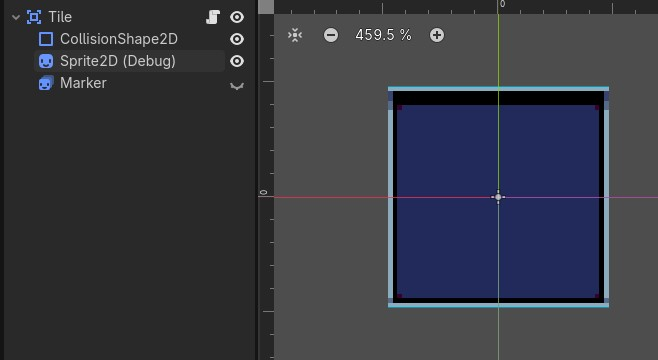
\includegraphics[width=0.85\textwidth]{../Imagenes/EjemploEscena}
	\caption{Estructura de la escena \texttt{Tile} en el editor de Godot}
	\label{fig:EjemploEscena}
\end{figure}

La comunicación entre nodos puede realizarse de tres formas. La primera es mediante \textbf{referencias directas}: un nodo obtiene acceso a otro con \texttt{GetNode()} y llama a sus métodos directamente. La segunda es mediante \textbf{señales}, el sistema de eventos nativo de Godot: un nodo emite una señal cuando ocurre algo relevante y otros nodos suscritos reaccionan sin necesidad de conocerse mutuamente. Para esta última he optado por utilizar los eventos de C\# estándar (event Action), utilizados para una comunicación más rápida y con tipado fuerte entre clases de lógica pura y controladores, reduciendo asi la dependencia con el editor de Godot. La tercera es mediante \textbf{clases	estáticas o instancias globales}, accesibles desde cualquier punto del código sin depender de la posición en el árbol. Una característica importante de Godot con C\# es que no toda clase tiene que ser un nodo: es válido definir clases C\# ordinarias que operen sobre los datos del árbol sin pertenecer a él, lo que permite aislar la lógica de negocio del ciclo de vida del motor.

La Figura~\ref{fig:GodotModelo} ilustra este modelo con un subconjunto representativo de los nodos del proyecto. No pretende recoger la totalidad del árbol de escenas, sino mostrar algunos tipos de nodos más relevantes, su jerarquía y algunos de los tres mecanismos de comunicación descritos.

\begin{figure}[H]
	\centering
	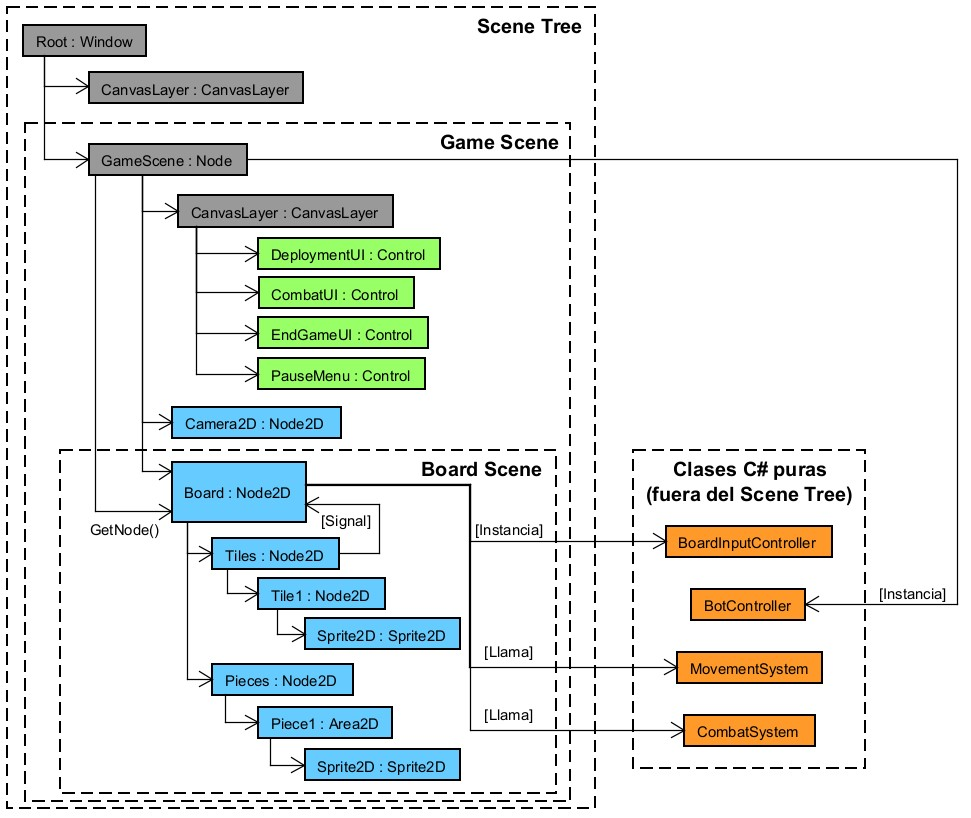
\includegraphics[width=0.85\textwidth]{../Imagenes/GodotModelo}
	\caption{Modelo de ejecución de Godot ilustrado con algunos nodos del proyecto.}
	\label{fig:GodotModelo}
\end{figure}

\subsection*{Arquitectura de NeuroForge}

Con este modelo en mente, el sistema se organiza en una \textbf{arquitectura en tres capas} que separa la representación visual de la lógica pura de juego y de los datos. Esta separación es una decisión de diseño para evitar que las reglas del juego queden entrelazadas con el código de renderizado o de interfaz.

La Figura~\ref{fig:ArquitecturaDelSistema} muestra una vista simplificada de los principales componentes de cada capa. Se incluyen los elementos más representativos de cada nivel.

\begin{figure}[H]
	\centering
	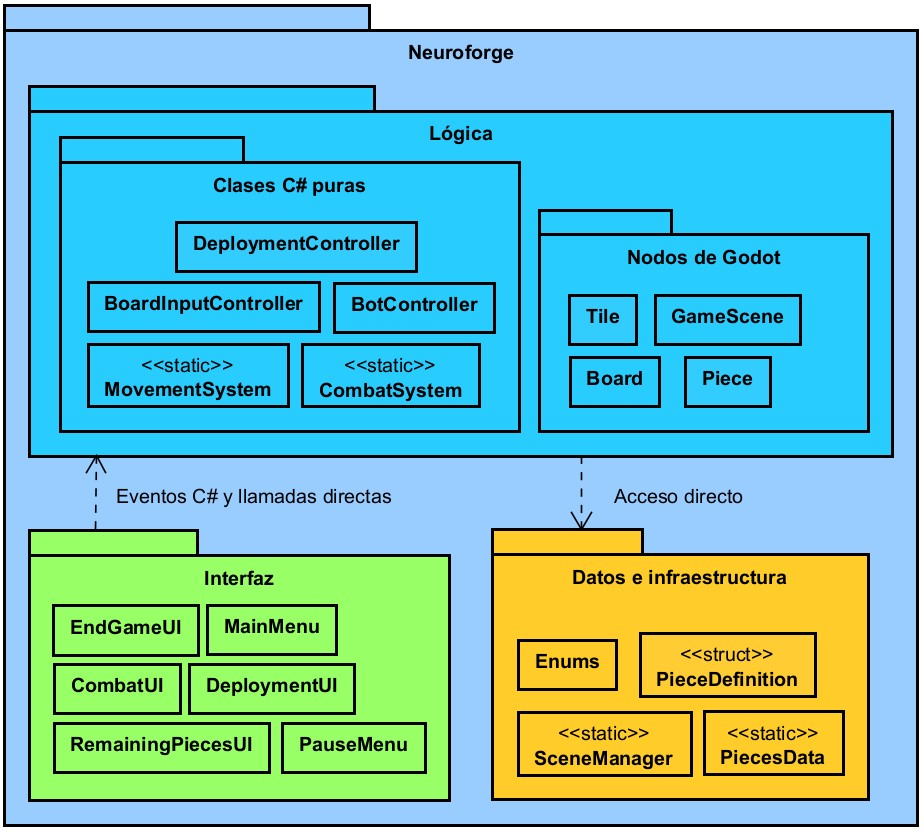
\includegraphics[width=\textwidth]{../Imagenes/ArquitecturaDelSistema}
	\caption{Vista simplificada de la arquitectura de NeuroForge en tres capas.}
	\label{fig:ArquitecturaDelSistema}
\end{figure}

La \textbf{capa de interfaz} agrupa todos los nodos que heredan de \texttt{Control}. Su responsabilidad se limita a capturar las intenciones del jugador y reflejar el estado del juego visualmente. Ninguno de estos nodos toma decisiones de lógica de juego: cuando el jugador pulsa un botón, la capa de presentación notifica a la capa inferior mediante eventos C\# estándar (\texttt{event Action}), y espera recibir los datos actualizados para refrescar la vista.

La \textbf{capa de lógica de juego} es el núcleo funcional del sistema. Aquí conviven dos tipos de clases con naturalezas distintas. \texttt{GameScene}, \texttt{Board}, \texttt{Tile} y \texttt{Piece} son nodos de Godot porque necesitan estar en el árbol de escenas para gestionar el input del ratón, coordinar animaciones y participar en el ciclo de vida del motor. Por otro lado, \texttt{BoardInputController}, \texttt{DeploymentController} y \texttt{BotController} son clases C\# puras creadas e instanciadas desde \texttt{GameScene} o \texttt{Board}, independientes del motor y por tanto más ligeras y fáciles de reutilizar. \texttt{MovementSystem} y \texttt{CombatSystem} son clases estáticas puras sin estado.

La \textbf{capa de datos e infraestructura} comprende los datos estáticos de configuración (\texttt{PiecesData}), el gestor de navegación entre escenas (\texttt{SceneManager}) y los enums que definen los valores del dominio (\texttt{GameState}, \texttt{PieceType}, \texttt{TileType}, etc.).

\subsection*{Comunicación entre capas}

Las tres capas se comunican siguiendo un flujo definido que evita dependencias circulares. La Figura~\ref{fig:comunicacion} muestra el flujo concreto que ocurre cuando el jugador confirma el despliegue de sus piezas e inicia la partida, ilustrando los dos mecanismos principales de comunicación: eventos C\# de presentación hacia lógica, y llamadas directas en el sentido contrario.

\begin{figure}[H]
	\centering
	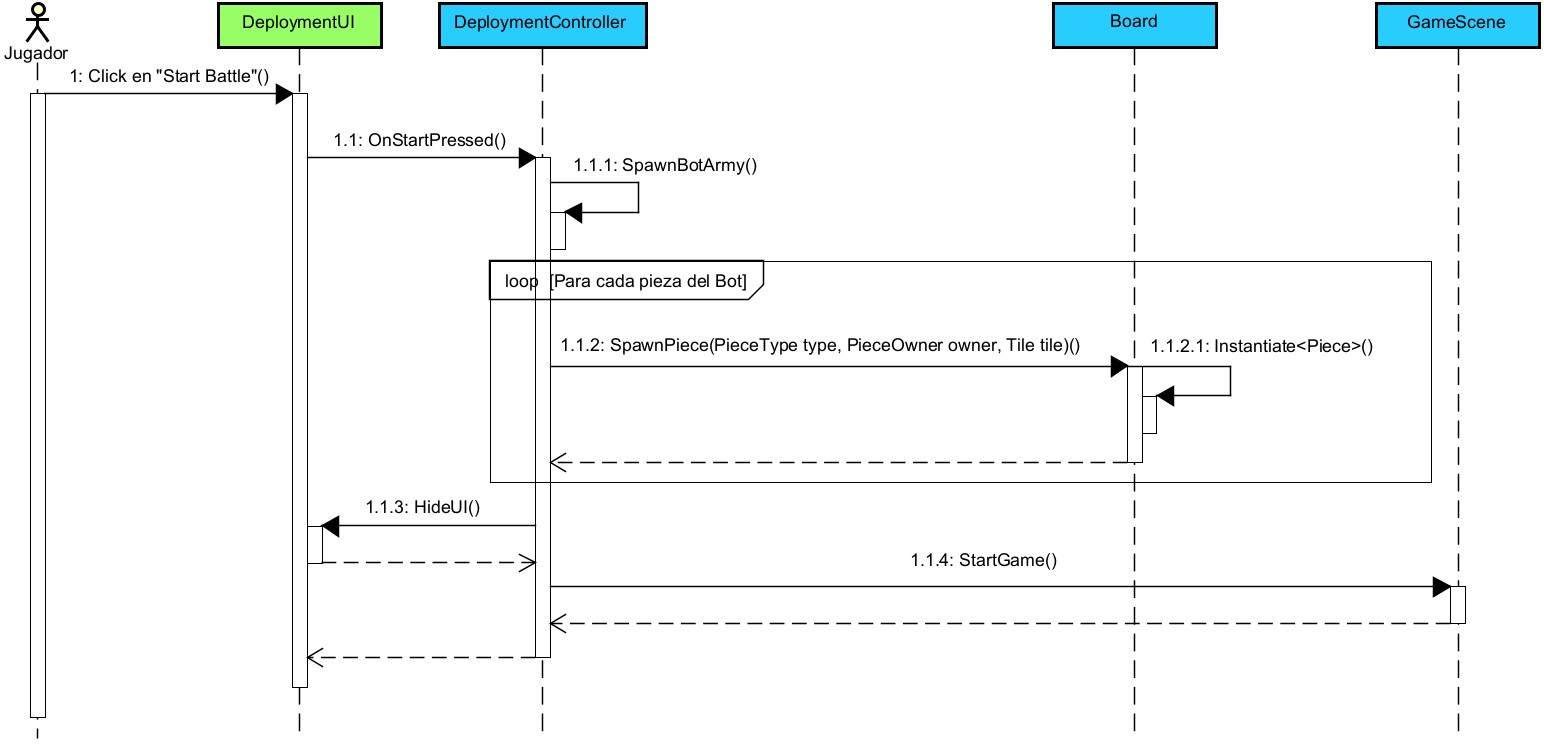
\includegraphics[width=\textwidth]{../Imagenes/ComunicacionEntreCapas}
	\caption{Ejemplo de comunicación entre capas durante la confirmación del despliegue.}
	\label{fig:ComunicacionEntreCapas}
\end{figure}

La presentación se comunica hacia la lógica mediante \textbf{eventos C\#}: \texttt{DeploymentUI} emite \texttt{OnStartPressed} sin conocer quién lo escucha. En sentido contrario, la lógica actualiza la presentación mediante \textbf{llamadas directas} a métodos de la UI como \texttt{HideUI()}. Dentro de la capa de lógica, \texttt{GameScene} previamente inyectó su propia referencia en \texttt{Board} mediante \texttt{Board.Initialize(this)} al momento de su creación, estableciendo un canal bidireccional controlado. La lógica accede a los datos mediante acceso directo a propiedades de \texttt{Tile} y \texttt{Piece}, o mediante consultas al diccionario estático de \texttt{PiecesData} por ejemplo.

% ─────────────────────────────────────────────────────────────────────────────
\section{Módulos o componentes del sistema}
% ─────────────────────────────────────────────────────────────────────────────

El sistema se divide en cinco módulos con responsabilidades claramente delimitadas. La Figura~\ref{fig:ComponentesDelSistema} muestra las dependencias entre ellos. Se representan los componentes principales de cada módulo; los detalles de implementación se describen en el texto que sigue.

\begin{figure}[H]
	\centering
	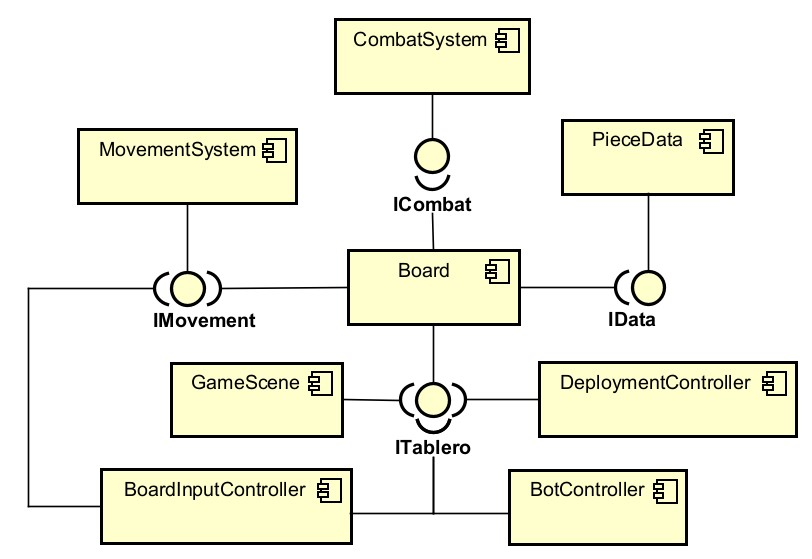
\includegraphics[width=0.85\textwidth]{../Imagenes/ComponentesDelSistema}
	\caption{Módulos del sistema y sus dependencias principales.}
	\label{fig:ComponentesDelSistema}
\end{figure}



\textbf{Módulo de orquestación.} Formado únicamente por \texttt{GameScene}, que actúa como gestor central del estado de la partida. Mantiene el turno activo y el estado mediante el enum \texttt{GameState} —con los valores \texttt{DEPLOYMENT}, \texttt{WAITING\_INPUT}, \texttt{EXECUTING\_ACTION}, \texttt{COMBAT} y \texttt{GAME\_OVER}— y coordina el resto de módulos. En su método \texttt{\_Ready()} instancia \texttt{Board}, \texttt{BotController} y \texttt{DeploymentController}, inyectando las referencias necesarias entre ellos. También gestiona la pausa mediante \texttt{GetTree().Paused}, mecanismo nativo de Godot que detiene el procesamiento de todos los nodos cuyo \texttt{ProcessMode} no esté configurado explícitamente como \texttt{Always}.

\textbf{Módulo de tablero.} Formado por \texttt{Board}, \texttt{Tile} y \texttt{BoardInputController}. \texttt{Board} genera la cuadrícula a partir del \texttt{TileMapLayer} en su método \texttt{\_Ready()}, e instancia \texttt{BoardInputController} en \texttt{Initialize()}. Es el punto de entrada de todo el input del tablero: cuando el jugador hace clic sobre una casilla, \texttt{Tile.\_InputEvent()} delega en \texttt{Board.OnTileClicked()}, que según el estado de la partida redirige la acción bien a \texttt{DeploymentController.TryTogglePiece()} durante el despliegue, bien a \texttt{BoardInputController.HandleTileClick()} durante la partida. \texttt{Board} también expone \texttt{MovePiece()} y \texttt{ResolveCombat()}, los dos métodos que modifican el estado físico del tablero.

\textbf{Módulo de piezas.} Compuesto por \texttt{Piece} y \texttt{PiecesData}. \texttt{Piece} encapsula tanto los datos de estado (tipo, rango, propietario, visibilidad) como la lógica visual: actualización del sprite mediante regiones del atlas y animaciones de movimiento y revelación. Gestiona además el historial de movimientos necesario para la restricción de oscilación entre 2 casillas. \texttt{PiecesData} centraliza todas las definiciones de piezas en un diccionario estático indexado por \texttt{PieceType}, evitando que valores de rango, cantidad máxima o columna de atlas queden dispersos por el código.

\textbf{Módulo de sistemas de juego.} Formado por las clases estáticas \texttt{MovementSystem} y \texttt{CombatSystem}. \texttt{MovementSystem} encapsula toda la lógica de validación de movimiento, incluyendo el movimiento especial del explorador (\texttt{IsScoutPathValid()}) y la restricción de oscilación entre dos casillas. \texttt{CombatSystem} aplica las reglas de combate en un único método \texttt{Resolve()}, con los casos especiales —torreta y phantom— resueltos mediante guardas explícitas antes de la regla general de rango. Al ser clases estáticas sin estado, pueden invocarse desde cualquier parte del código sin efectos secundarios, lo que resulta especialmente valioso de cara a la simulación de partidas en la iteración~4.

\textbf{Módulo de bot y despliegue.} Formado por \texttt{BotController} y \texttt{DeploymentController}, ambas clases C\# puras creadas por \texttt{GameScene}. \texttt{BotController} recibe una referencia a \texttt{Board} en su constructor y, cuando \texttt{GameScene} invoca \texttt{PlayTurn()}, obtiene la lista de acciones posibles mediante \texttt{Board.GetAllPossibleActions()}, selecciona una y la ejecuta mediante \texttt{Board.ExecuteBotAction()}. \texttt{DeploymentController} se suscribe a los eventos de \texttt{DeploymentUI} y gestiona tanto la colocación manual de piezas del jugador (a través de \texttt{TryTogglePiece()}, invocado por \texttt{Board}) como la generación aleatoria del ejército del bot y el inicio de la partida mediante \texttt{StartBattle()}.

% ─────────────────────────────────────────────────────────────────────────────
\section{Diseño de clases}
% ─────────────────────────────────────────────────────────────────────────────

% ─────────────────────────────────────────────────────────────────────────────
\section{Diseño de interfaz de usuario}
% ─────────────────────────────────────────────────────────────────────────────

% ─────────────────────────────────────────────────────────────────────────────
\section{Patrones de diseño aplicados}
% ─────────────────────────────────────────────────────────────────────────────

% ─────────────────────────────────────────────────────────────────────────────
\section{Seguridad y rendimiento}
% ─────────────────────────────────────────────────────────────────────────────
